\section{Översikt av system}
Plattformen består av sammanlagt fyra enheter. En PC-enhet, en huvudenhet, en sensorenhet och en styrenhet. \\
PC-enheten är framförallt ett användargränssnitt som gör det enkelt för användaren att styra roboten och robotarmen men fungerar även som ett debugverktyg där användaren kan se robotens status och debuginformation. Huvudenheten står för huvuddelen av alla beräkningar roboten behöver göra så som regleringsalgoritm för linjeföljaren och koordinatkonvertering för armen. Sensorenheten innehåller den funktionalitet som krävs för att driva alla systemets sensorer och styrenheten innehåller den funktionalitet som krävs för att köra motorer och servon.

\subsection{Kommunikationskanaler}
I det fall att roboten arbetar i manuellt läge, skickar PC-enheten kommandon till huvudenheten över Blåtand. I annat fall arbetar roboten autonomt och PC-enheten skickar endast förfrågningar angående robotens status. Huvudenheten skickar kommandon till sensorenheten och styrenheten över en SPI-buss.

\subsection{Uppgraderbarhet}
Kommunikation mellan huvudmodulen och PC-enheten kommer att ske över Blåtand och kommer att användas för att sätta upp ett PAN. Över denna sätts en TCP/IP anslutning upp och data skickas över en Python-socket vilket leder till att bluetooth kan bytas ut mot till exempel WIFI, en ethernetkabel eller annan överföringskanal som tillåter TCP/IP. \\
Kommunikationen mellan huvudmodulen och styrenheten samt sensormodulen sker över en SPI-buss med ett väldefinierat protokoll. Om det önskas kan sensormodulen och styrmodulen bytas ut mot andra moduler så länge de använder samma protokoll. Styrenheten kommunicerar med servona över UART och använder ett protokoll speciellt för Trossenrobotics Reactor vilket leder till att armen inte kan bytas ut mot någon annan.

\begin{figure}[h!]
\center
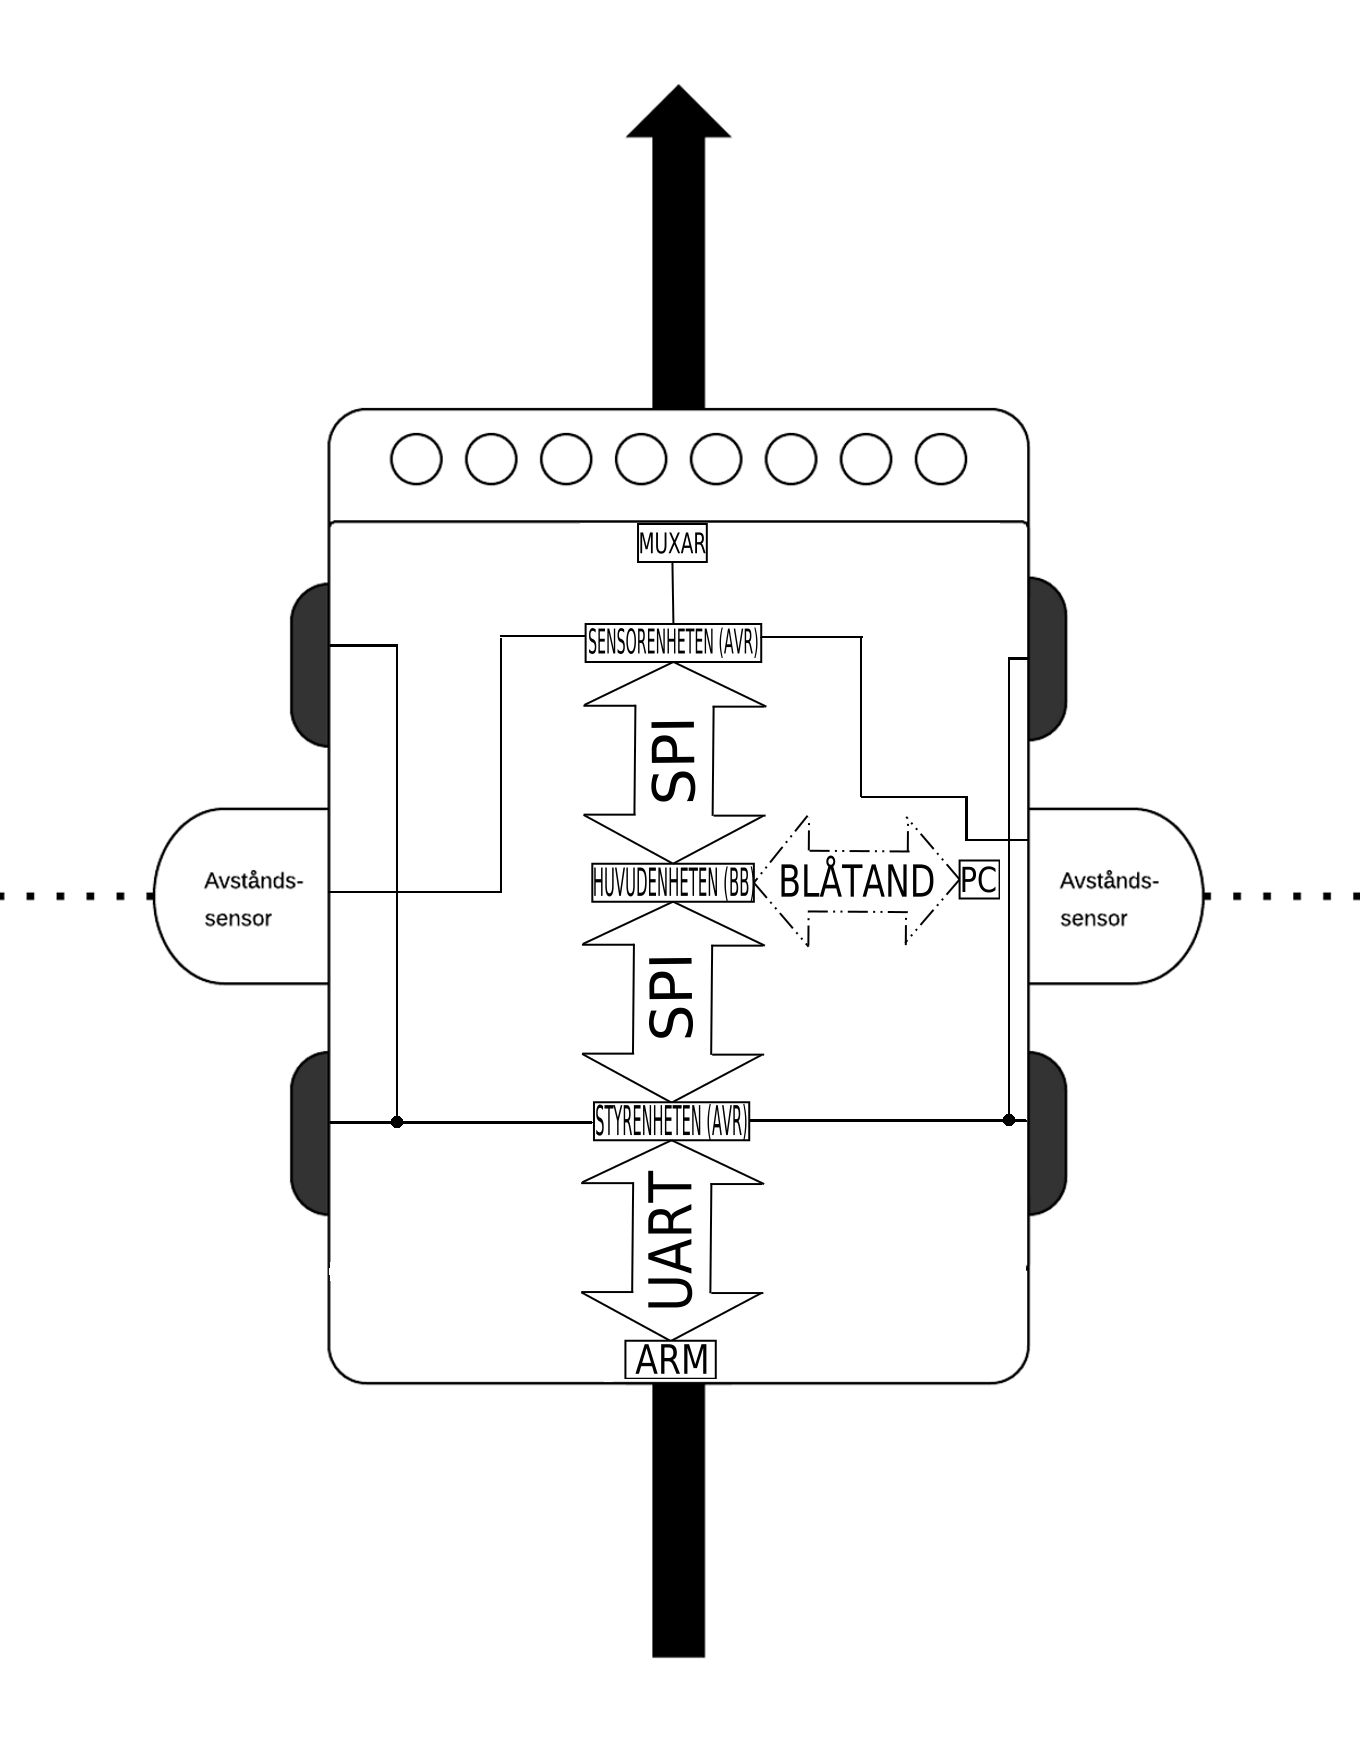
\includegraphics[scale=0.32]{grafik/robot}
\caption{Översikt över roboten} \label{designspec:robot}
\end{figure}
